% Options for packages loaded elsewhere
\PassOptionsToPackage{unicode}{hyperref}
\PassOptionsToPackage{hyphens}{url}
\PassOptionsToPackage{dvipsnames,svgnames,x11names}{xcolor}
%
\documentclass[
  letterpaper,
  DIV=11,
  numbers=noendperiod,
  oneside]{scrartcl}

\usepackage{amsmath,amssymb}
\usepackage{iftex}
\ifPDFTeX
  \usepackage[T1]{fontenc}
  \usepackage[utf8]{inputenc}
  \usepackage{textcomp} % provide euro and other symbols
\else % if luatex or xetex
  \usepackage{unicode-math}
  \defaultfontfeatures{Scale=MatchLowercase}
  \defaultfontfeatures[\rmfamily]{Ligatures=TeX,Scale=1}
\fi
\usepackage{lmodern}
\ifPDFTeX\else  
    % xetex/luatex font selection
\fi
% Use upquote if available, for straight quotes in verbatim environments
\IfFileExists{upquote.sty}{\usepackage{upquote}}{}
\IfFileExists{microtype.sty}{% use microtype if available
  \usepackage[]{microtype}
  \UseMicrotypeSet[protrusion]{basicmath} % disable protrusion for tt fonts
}{}
\makeatletter
\@ifundefined{KOMAClassName}{% if non-KOMA class
  \IfFileExists{parskip.sty}{%
    \usepackage{parskip}
  }{% else
    \setlength{\parindent}{0pt}
    \setlength{\parskip}{6pt plus 2pt minus 1pt}}
}{% if KOMA class
  \KOMAoptions{parskip=half}}
\makeatother
\usepackage{xcolor}
\usepackage[left=1in,marginparwidth=2.0666666666667in,textwidth=4.1333333333333in,marginparsep=0.3in]{geometry}
\setlength{\emergencystretch}{3em} % prevent overfull lines
\setcounter{secnumdepth}{-\maxdimen} % remove section numbering
% Make \paragraph and \subparagraph free-standing
\makeatletter
\ifx\paragraph\undefined\else
  \let\oldparagraph\paragraph
  \renewcommand{\paragraph}{
    \@ifstar
      \xxxParagraphStar
      \xxxParagraphNoStar
  }
  \newcommand{\xxxParagraphStar}[1]{\oldparagraph*{#1}\mbox{}}
  \newcommand{\xxxParagraphNoStar}[1]{\oldparagraph{#1}\mbox{}}
\fi
\ifx\subparagraph\undefined\else
  \let\oldsubparagraph\subparagraph
  \renewcommand{\subparagraph}{
    \@ifstar
      \xxxSubParagraphStar
      \xxxSubParagraphNoStar
  }
  \newcommand{\xxxSubParagraphStar}[1]{\oldsubparagraph*{#1}\mbox{}}
  \newcommand{\xxxSubParagraphNoStar}[1]{\oldsubparagraph{#1}\mbox{}}
\fi
\makeatother


\providecommand{\tightlist}{%
  \setlength{\itemsep}{0pt}\setlength{\parskip}{0pt}}\usepackage{longtable,booktabs,array}
\usepackage{calc} % for calculating minipage widths
% Correct order of tables after \paragraph or \subparagraph
\usepackage{etoolbox}
\makeatletter
\patchcmd\longtable{\par}{\if@noskipsec\mbox{}\fi\par}{}{}
\makeatother
% Allow footnotes in longtable head/foot
\IfFileExists{footnotehyper.sty}{\usepackage{footnotehyper}}{\usepackage{footnote}}
\makesavenoteenv{longtable}
\usepackage{graphicx}
\makeatletter
\newsavebox\pandoc@box
\newcommand*\pandocbounded[1]{% scales image to fit in text height/width
  \sbox\pandoc@box{#1}%
  \Gscale@div\@tempa{\textheight}{\dimexpr\ht\pandoc@box+\dp\pandoc@box\relax}%
  \Gscale@div\@tempb{\linewidth}{\wd\pandoc@box}%
  \ifdim\@tempb\p@<\@tempa\p@\let\@tempa\@tempb\fi% select the smaller of both
  \ifdim\@tempa\p@<\p@\scalebox{\@tempa}{\usebox\pandoc@box}%
  \else\usebox{\pandoc@box}%
  \fi%
}
% Set default figure placement to htbp
\def\fps@figure{htbp}
\makeatother
% definitions for citeproc citations
\NewDocumentCommand\citeproctext{}{}
\NewDocumentCommand\citeproc{mm}{%
  \begingroup\def\citeproctext{#2}\cite{#1}\endgroup}
\makeatletter
 % allow citations to break across lines
 \let\@cite@ofmt\@firstofone
 % avoid brackets around text for \cite:
 \def\@biblabel#1{}
 \def\@cite#1#2{{#1\if@tempswa , #2\fi}}
\makeatother
\newlength{\cslhangindent}
\setlength{\cslhangindent}{1.5em}
\newlength{\csllabelwidth}
\setlength{\csllabelwidth}{3em}
\newenvironment{CSLReferences}[2] % #1 hanging-indent, #2 entry-spacing
 {\begin{list}{}{%
  \setlength{\itemindent}{0pt}
  \setlength{\leftmargin}{0pt}
  \setlength{\parsep}{0pt}
  % turn on hanging indent if param 1 is 1
  \ifodd #1
   \setlength{\leftmargin}{\cslhangindent}
   \setlength{\itemindent}{-1\cslhangindent}
  \fi
  % set entry spacing
  \setlength{\itemsep}{#2\baselineskip}}}
 {\end{list}}
\usepackage{calc}
\newcommand{\CSLBlock}[1]{\hfill\break\parbox[t]{\linewidth}{\strut\ignorespaces#1\strut}}
\newcommand{\CSLLeftMargin}[1]{\parbox[t]{\csllabelwidth}{\strut#1\strut}}
\newcommand{\CSLRightInline}[1]{\parbox[t]{\linewidth - \csllabelwidth}{\strut#1\strut}}
\newcommand{\CSLIndent}[1]{\hspace{\cslhangindent}#1}

\KOMAoption{captions}{tableheading}
\makeatletter
\@ifpackageloaded{caption}{}{\usepackage{caption}}
\AtBeginDocument{%
\ifdefined\contentsname
  \renewcommand*\contentsname{Table of contents}
\else
  \newcommand\contentsname{Table of contents}
\fi
\ifdefined\listfigurename
  \renewcommand*\listfigurename{List of Figures}
\else
  \newcommand\listfigurename{List of Figures}
\fi
\ifdefined\listtablename
  \renewcommand*\listtablename{List of Tables}
\else
  \newcommand\listtablename{List of Tables}
\fi
\ifdefined\figurename
  \renewcommand*\figurename{Figure}
\else
  \newcommand\figurename{Figure}
\fi
\ifdefined\tablename
  \renewcommand*\tablename{Table}
\else
  \newcommand\tablename{Table}
\fi
}
\@ifpackageloaded{float}{}{\usepackage{float}}
\floatstyle{ruled}
\@ifundefined{c@chapter}{\newfloat{codelisting}{h}{lop}}{\newfloat{codelisting}{h}{lop}[chapter]}
\floatname{codelisting}{Listing}
\newcommand*\listoflistings{\listof{codelisting}{List of Listings}}
\makeatother
\makeatletter
\makeatother
\makeatletter
\@ifpackageloaded{caption}{}{\usepackage{caption}}
\@ifpackageloaded{subcaption}{}{\usepackage{subcaption}}
\makeatother
\makeatletter
\@ifpackageloaded{sidenotes}{}{\usepackage{sidenotes}}
\@ifpackageloaded{marginnote}{}{\usepackage{marginnote}}
\makeatother

\usepackage{bookmark}

\IfFileExists{xurl.sty}{\usepackage{xurl}}{} % add URL line breaks if available
\urlstyle{same} % disable monospaced font for URLs
\hypersetup{
  pdftitle={4: Meaning},
  colorlinks=true,
  linkcolor={blue},
  filecolor={Maroon},
  citecolor={Blue},
  urlcolor={Blue},
  pdfcreator={LaTeX via pandoc}}


\title{4: Meaning}
\author{}
\date{}

\begin{document}
\maketitle


\section{What is ``Meaning'' and why is it so important to
Sociology?}\label{what-is-meaning-and-why-is-it-so-important-to-sociology}

Look at this illustration.\sidenote{\footnotesize This illusion is the famous ``rabbit
  and duck'' illustration, originally
  \href{https://en.wikipedia.org/wiki/Rabbit\%E2\%80\%93duck_illusion}{from}
  an 1884 German Newspaper, which is commonly used to demonstrate the
  ``gestalt shift'' in psychology by which the illustration's appearance
  suddenly shifts from ``being'' a rabbit to ``being'' a duck.} What do
you see?

\begin{figure}[H]

{\centering \pandocbounded{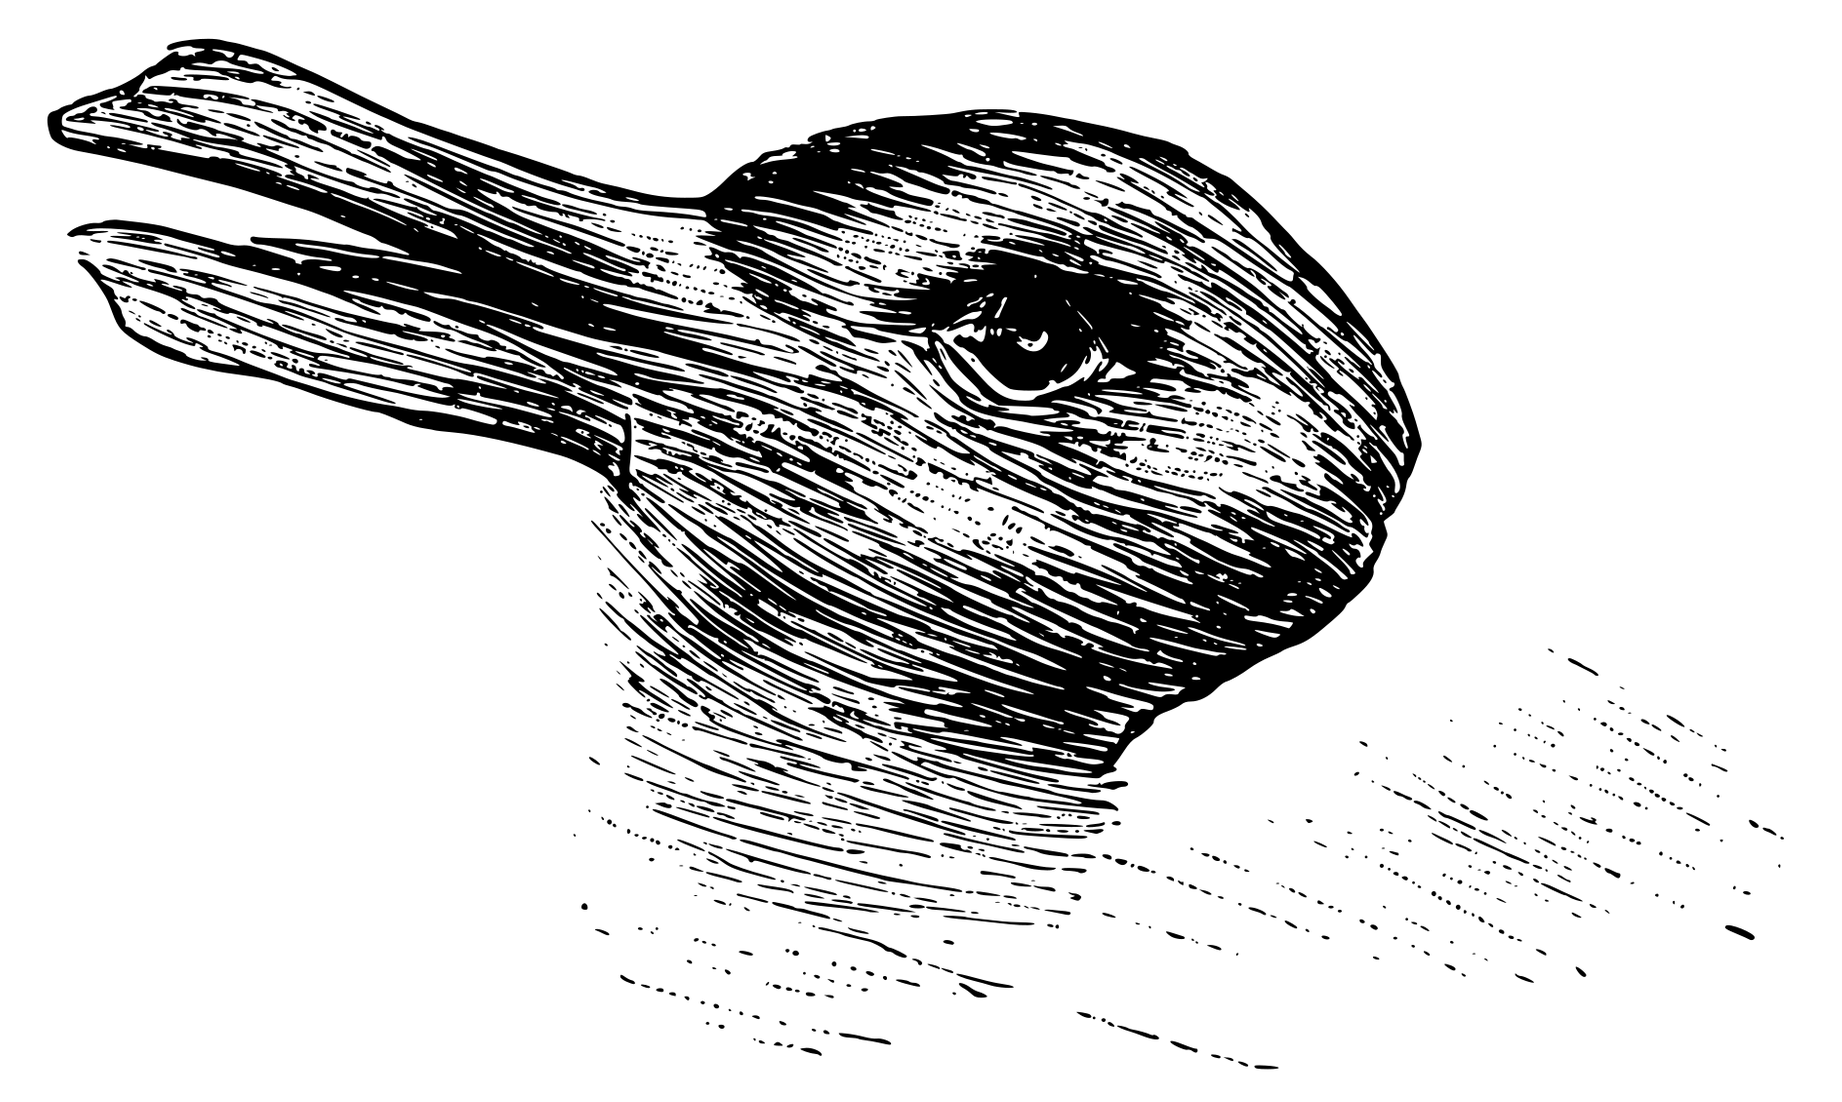
\includegraphics[keepaspectratio]{../images/4_rabbit_and_duck.png}}

}

\caption{An Optical Illusion}

\end{figure}%

Some people see a rabbit. Some see a duck. Some see something in
between. But what matters for us here is not exactly \emph{what} you
saw, but \emph{that} you saw something in the first place. Someone,
inspired perhaps by a rabbit or a duck, made an illustration with a pen
and their hand, then that was scanned digitally and it now \emph{is}
only an arrangment of pixels on your screen. But your brain was able to
take that arrangement of pixels and integrate it into a symbol
representing something else, namely, a rabbit (or duck, or something in
between). Sociologists (and other social scientists and humanities
scholars) summarize this action of your brain to integrate stimuli into
references to something else out ability to perceive \textbf{meaning} or
\textbf{significance} in the world.

Sociologists care so much about meaning for a few reasons, but the most
central relates to social constructions. Recall that social
constructions are just real phemonena in the world which exist by virtue
of our shared acceptance that the exist. That word \emph{shared} is the
key: for \emph{how can it be} that we manage to arrive at the same, or
even just similar, collective (or at least intersubjective)
understandings of what is happening? A theory of meaning provides the
answer--it is the ability to arrive at a shared understanding of what a
thing, social setting, or phenomenon is ``about,'' at least enough so to
enable communication.

As we discussed in the \href{../chapters/Ch_3_Method.qmd}{last unit},
when discussing Symbolic Interactionism, the meanings we find in symbols
have a general structure: that of a \textbf{symbol}. A symbol is
composed of two parts: the \textbf{signifier}, which is the thing that
is doing the representing, and the \textbf{signified}, which is the
meaning or significance being represented. Sometimes, the relationship
between signifier and signfied is \emph{iconic}, which is to say, one of
direct resemblance. This is most famous in some languages, like
\href{https://en.wikipedia.org/wiki/Egyptian_hieroglyphs}{ancient
Egyptian hieroglyphics}. But there are also times where meaning is
highly dependent on its contextual appearance among other symbols. Most
modern languages follow this more complex pattern.

Sociologists tend to study these complex objects, symbols, and their
meaning at two levels of analysis, the micro and macro.

\subsubsection{Micro-Analysis of
Culture}\label{micro-analysis-of-culture}

At the micro level, going back to the beginning of the sociological
tradition (this time to a sociologist named Max Weber, who also
theorized ``rationalization''), sociologists have seen a tight coupling
of meaning and action together. Indeed, Weber saw them as identical: for
a person to ``act'' (which is to say, do something), was for them to

\begin{quote}
{[}attach{]} subjective meaning to his behavior---be it overt or covert,
omission or acquiesence. Action is `social' insofar as its subjective
meaning takes account of the behavior of others and is thereby oriented
in its course\ldots in no case does {[}meaning{]} refer to an
objectively `correct' meaning or one whihc is `true' in some
metaphysical sense (Weber
1978:4)\marginpar{\begin{footnotesize}
\begin{CSLReferences}{2}{0}
\bibitem[\citeproctext]{ref-weberEconomySociety1978}
Weber, Max. 1978. \emph{Economy and {Society}}. Berkeley: University of
California.
\end{CSLReferences}
\vspace{2mm}\par\end{footnotesize}}.
\end{quote}

\texttt{Start\ with\ Weber\textquotesingle{}s\ basic\ sociological\ terms.}

\texttt{How\ do\ meanings\ motivate\ and\ justify\ action\ for\ people\ and\ groups?}

\subsubsection{Macro-Analysis of
Culture}\label{macro-analysis-of-culture}

\texttt{Starts\ with\ Durkheim\textquotesingle{}s\ views\ from\ the\ duality\ of\ human\ nature.}

\texttt{Asks\ how\ meanings\ are\ structured\ in\ relationship\ to\ one\ another,\ and\ how\ they\ mutate\ and\ change\ over\ time\ in\ complex\ societies.}

\texttt{Study\ the\ overall\ social\ function\ of\ some\ meanings\ vs\ others\ and\ their\ sociostructural\ outcomes.}

\texttt{The\ composition\ of\ meaning\ into\ symbols,\ made\ of\ signifier\ and\ signfied.\ \ In\ simple\ cases,\ what\ is\ signified\ is\ a\ concrete,\ material\ entity\ in\ the\ world.\ \ In\ a\ great\ number\ of\ other\ cases,\ however,\ what\ is\ signified\ by\ a\ symbol\ is\ *not*\ concrete,\ as\ in\ the\ concepts\ of\ a\ "market"\ or\ "love."}

\subsection{Meaning as unifying}\label{meaning-as-unifying}

\texttt{it\ is\ difficult\ to\ overstate\ the\ imporance\ of\ culture\ and\ meaning\ to\ the\ conduct\ of\ your\ everyday\ life.\ \ It\ is\ there\ that\ all\ information\ is\ stored\ that\ literally\ keeps\ you\ alive,\ and\ allows\ you\ to\ interact\ with\ society.}

\subsection{Meaning as a source of conflict and a vector for
power}\label{meaning-as-a-source-of-conflict-and-a-vector-for-power}

\texttt{But\ from\ very\ on\ in\ human\ history,\ culture\ has\ also\ been\ a\ way\ to\ (intentionally\ or\ not)\ establish\ boundaries\ and\ legitimate\ domination.}

\texttt{One\ "natural"\ source\ of\ conflict\ around\ culture\ is\ **polysemy**,\ or\ the\ fact\ that\ particular\ symbols\ can\ be\ interpreted\ in\ a\ variety\ of\ ways.}

\section{Cultural Universals}\label{cultural-universals}

\subsection{Marriage}\label{marriage}

\subsection{Property Rights}\label{property-rights}

\subsection{Religious Ritual}\label{religious-ritual}

\subsection{Language}\label{language}

\section{A brief history of civilization with a specific focus on
culture}\label{a-brief-history-of-civilization-with-a-specific-focus-on-culture}

The best evidence we have for the origins of sophisticated human culture
are around 50,000 ``BP'' (so, 48,000 years BCE or so), when there was
sudden, rapid evolution of human's burial practices, use of technology,
collective hunting practices, and even cultural artifacts like cave
paintings
(\textbf{aubertPalaeolithicCaveArt2018?})\marginpar{\begin{footnotesize}aubertPalaeolithicCaveArt2018\vspace{2mm}\par\end{footnotesize}}.\sidenote{\footnotesize There
  is considerable debate among archaeologists about whether this
  emergence was gradual or a ``sudden leap'' constituting a new phase of
  evolution.}

For about 40,000 years, nothing happened.\sidenote{\footnotesize This is a
  \href{https://getyarn.io/yarn-clip/6c7a19d7-d428-456e-b8d1-29ae296660a6}{Simpson's
  joke} that only your grandparents are aware of.} Then the last global
ice age (which began around 110,000 BP) ended, which both cut off the
Americas from the rest of the world (by flooding what is now the Bering
Strait between Siberia and Alaska), and also led to more favorable
climactic conditions for the domestication of animals and plants by
humans. Accordingly, pockets of durable human settlement--even, by 8 to
6,000 years BP, growing to the size of modest towns today.\sidenote{\footnotesize Estimates
  of one of the earliest human settlements, in Turkey, suggest it was
  populated by around 600 to 800 people
  (\textbf{kuijtHowManyPeople2024?}).\linebreak\linebreakkuijtHowManyPeople2024\linebreak}

\begin{figure}[H]

{\centering \pandocbounded{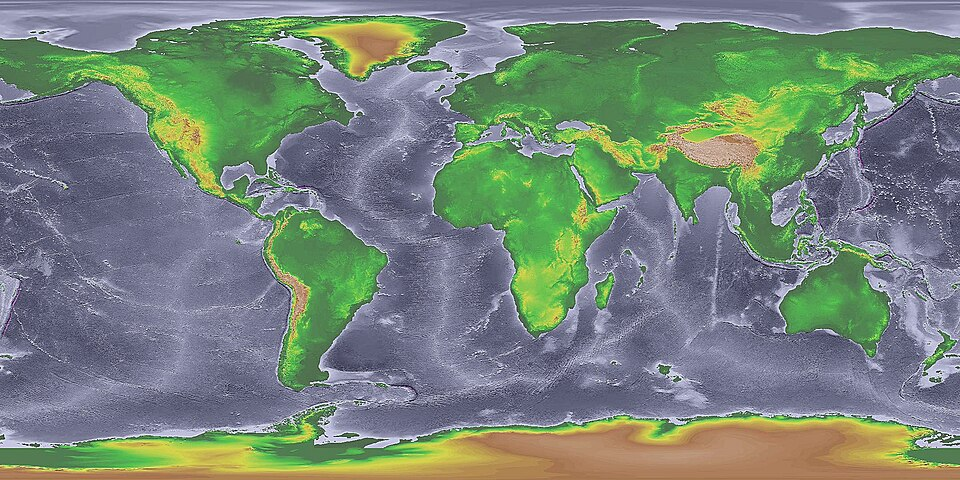
\includegraphics[keepaspectratio]{../images/4_Global_sea_levels_during_the_last_Ice_Age.jpg}}

}

\caption{The last global ice age vastly \emph{lowered} sea levels,
making land much more connected than it is today
(\href{https://en.wikipedia.org/wiki/Last_Glacial_Period\#/media/File:Global_sea_levels_during_the_last_Ice_Age.jpg.}{Source})}

\end{figure}%

Residing in cities meant that all aspects of human life gained a more
durable base, including human culture. The next major innovation was the
invention of \emph{writing,} or the ability to make human linguistic
expression \emph{durable} and \emph{distributable} across distances. The
first
\href{https://en.wikipedia.org/wiki/History_of_writing\#Emergence}{evidence
of writing} comes from Mesopotamia around 5000 years BP, and the
consensus is that it emerged independently in at least four places:
Mesopotamia, Mesoameria, China, and Egypt.

For our purposes of a sociological history of culture, however, it is
important to note that \emph{almost no one} outside of religious and
government officials could read or write until very recently.

\begin{figure}[H]

{\centering \pandocbounded{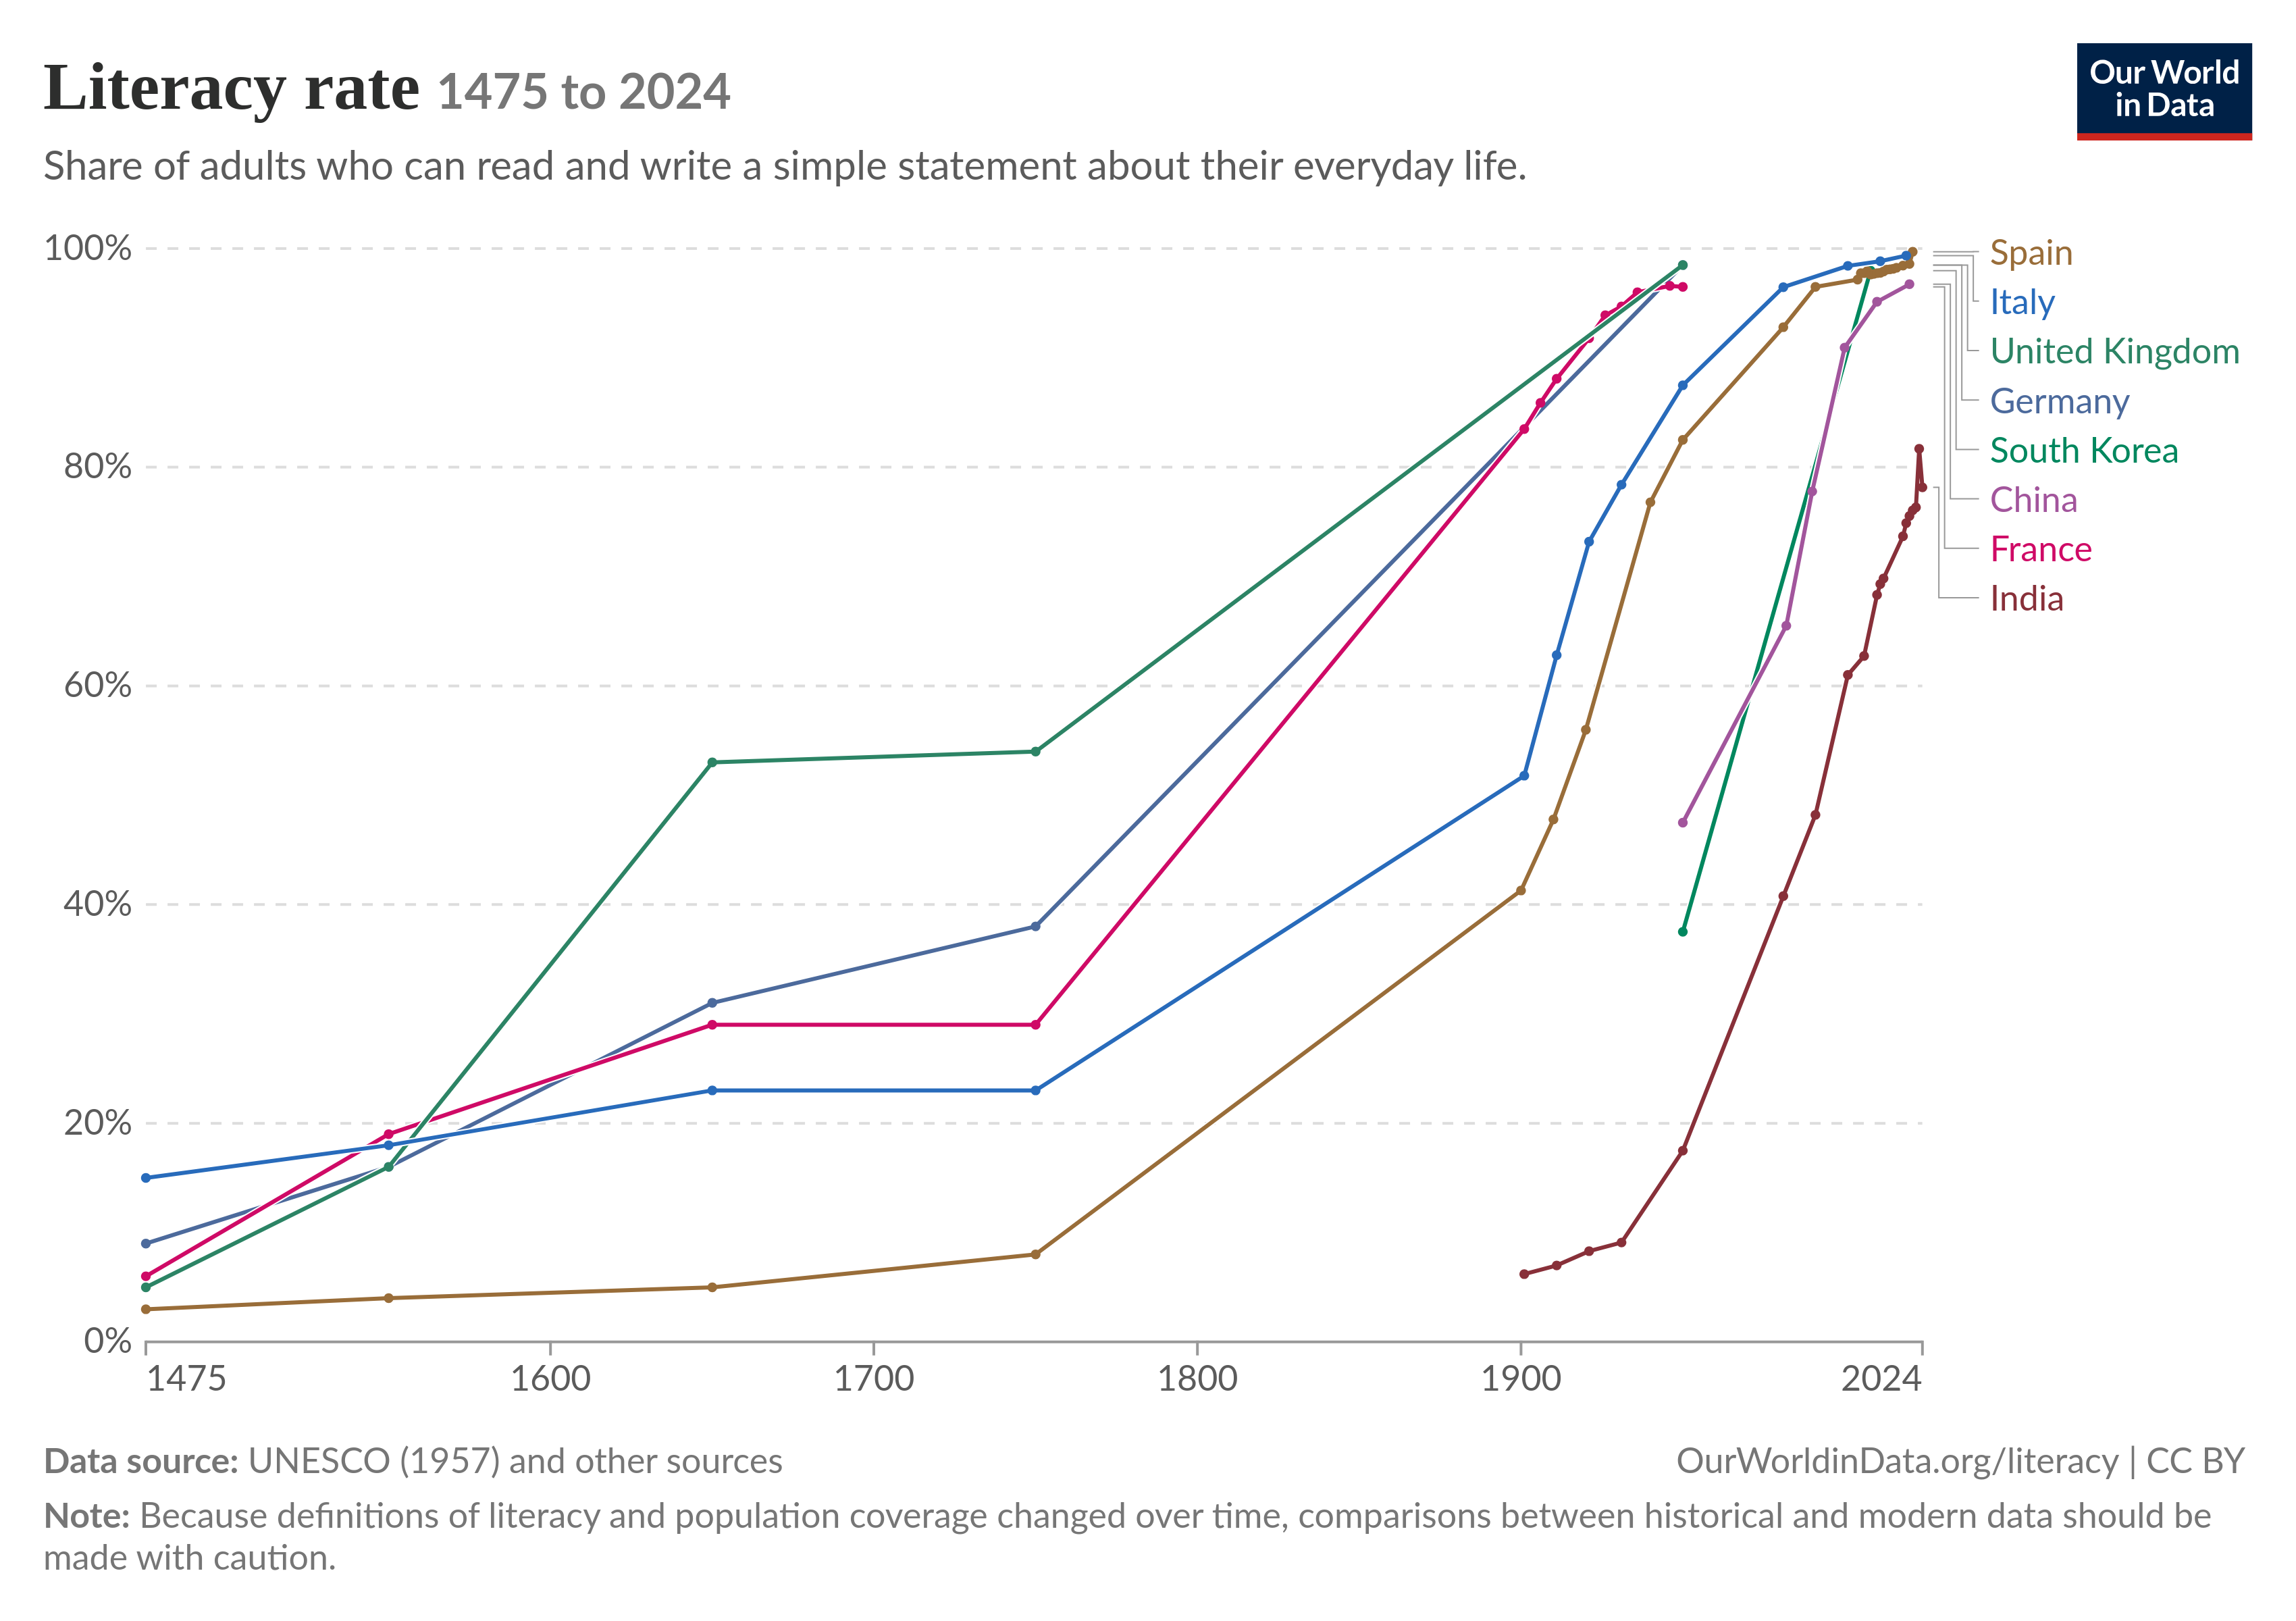
\includegraphics[keepaspectratio]{../images/4_cross-country-literacy-rates.png}}

}

\caption{Literacy rates (including historical esitmates) for the last
500 years among selected countries.}

\end{figure}%

Roughly on the same time scale (but accelerating more recently, afte the
last two hundred years or so) as the emergence of mass literacy, human
societies also experienced the rise and global dominance of
industrialization. This was organized accordingly to variety of logics
(the two most famous families are capitalism and communism), but its key
effect from a structural standpoint for the history of human culture was
to mechanize agriculture, thus \emph{vastly} reducing the number of
people who had to work to grow food for everyone else.

\begin{figure}[H]

{\centering \pandocbounded{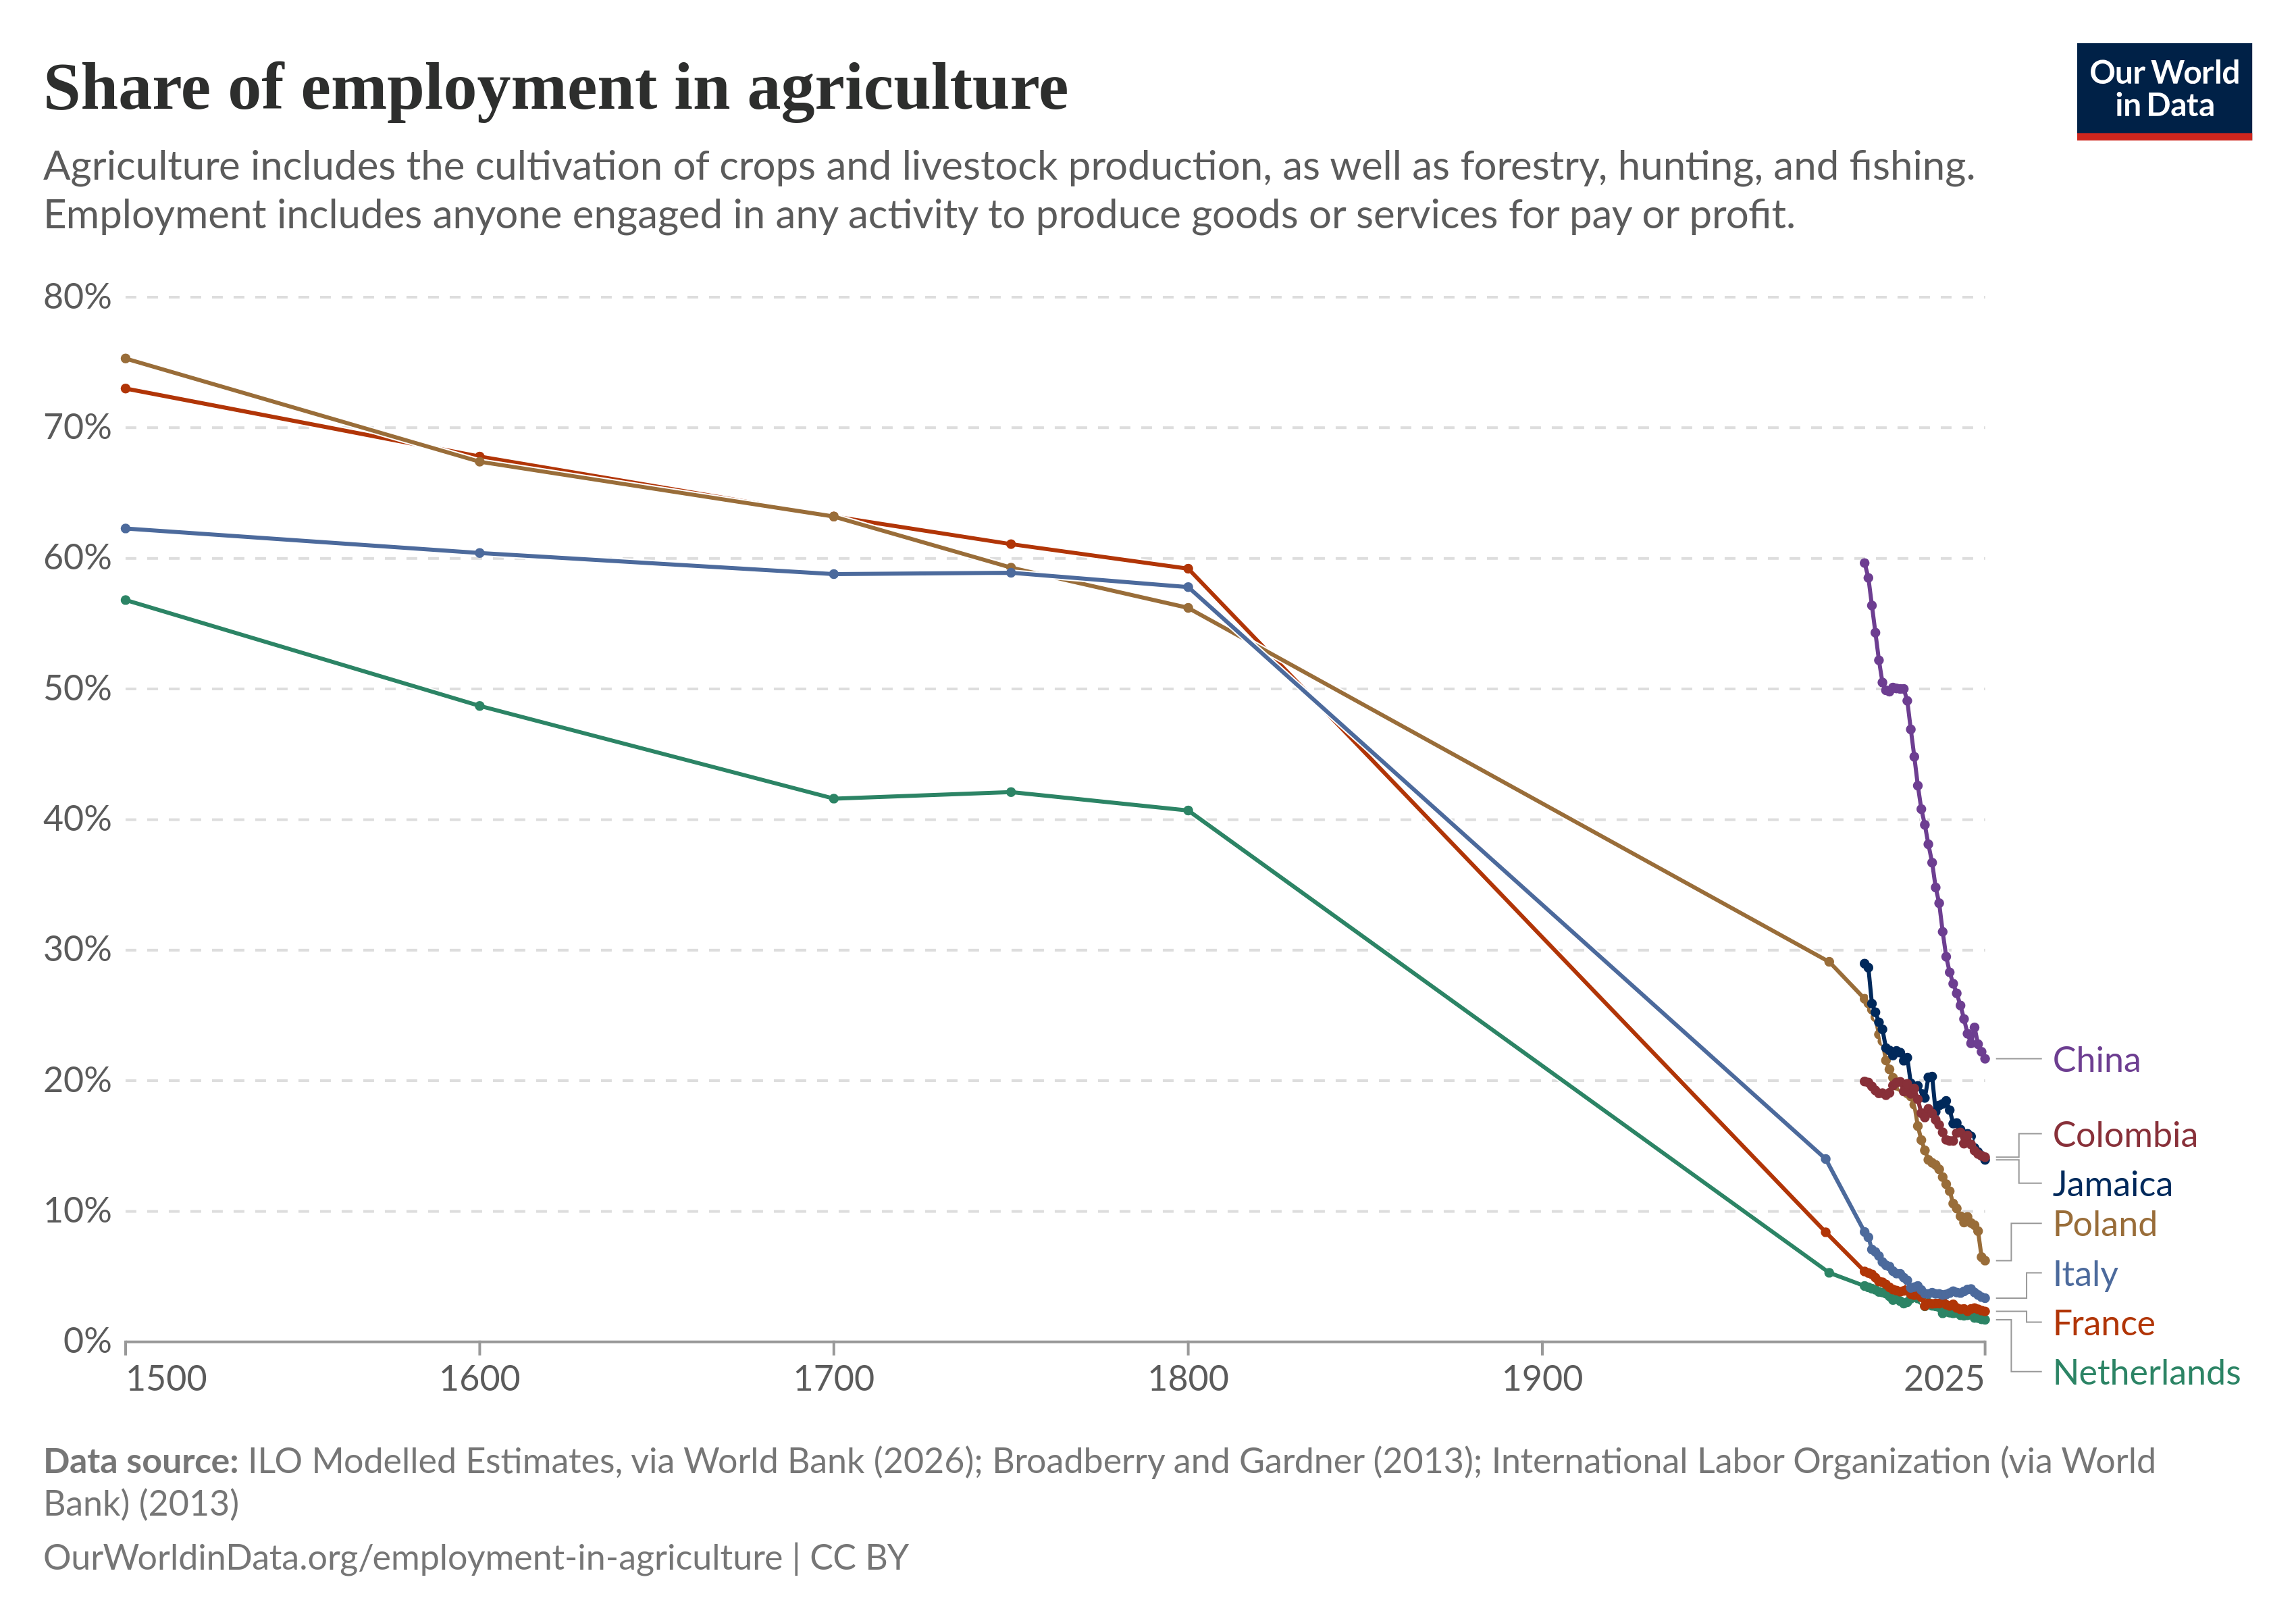
\includegraphics[keepaspectratio]{../images/4_share-of-employment-in-agriculture.png}}

}

\caption{The share of employment in agriculture, from 1475 to 2025.}

\end{figure}%

A final coda to our history of human culture: the emergence of mass
literacy, until the recent past, was organized around a
\textbf{broadcast} model, in which some central authority made decisions
(say, TV network executives) about what would be broadcast, and then
consumers received that product. Today, we may well have fragmented into
a much more \textbf{networked} dynamic, in which culture is distributed
along a series of channels that provide much more tailored messages and
meanings than we previously possible.

\section*{Cultural Dynamics today}\label{cultural-dynamics-today}
\addcontentsline{toc}{section}{Cultural Dynamics today}





\end{document}
